\chapter{Unity}
\label{chap:unity}

Dans cette partie, il s'agira finalement de parler du développement du module \texttt{Unity} utilisant la nouvelle plateforme mise en place, dont il est question Chapitre~\ref{chap:protoHP}. Ce développement fut la parfaite occasion de tester, de mettre à l'épreuve cette dernière et d'avoir, par la même occasion, un retour réel sur son utilisabilité. 

Dans un premier temps, nous discuterons des apports, des enjeux, mais aussi de la conception et de la cible du module. Nous en profiterons pour aborder les difficultés rencontrées, qu'elles soient liées à \texttt{Unity} où à la nouvelle plateforme. Dans un second temps, nous nous attarderons sur le développement d'une application avec ce module, de façon à évaluer s'il répond aux besoins et s'il y répond de façon efficace. Pour finir, nous effectuerons une rapide comparaison entre la version actuelle et la version en développement des kits (\texttt{Unity} et \texttt{Processing}), afin d'avoir une évaluation dans des conditions réelles d'utilisation et peut être faire émerger des pistes d'amélioration de la version \texttt{Unity}.

\section{Module Unity}

L'objectif du module \texttt{Unity} est de permettre à ses utilisateurs d'exploiter la puissance (logicielle et matérielle) de \texttt{Nectar} de façon intuitive, afin qu'ils puissent développer des applications de réalité augmentée spatiale sans jamais avoir besoin de se soucier des problèmes liés à cette technologie, comme la problématique de calibration du couple caméra projecteur par exemple.
Pour cela, nous avons créé dans \texttt{Unity} les composants et les comportements cruciaux du système tels que les caméras, les caméras de profondeur, les projecteurs, les utilisateurs, la table, et bien d'autres. En plus de résoudre bon nombre de problèmes pour l'utilisateur, ces composants rendent possible la représentation du monde réel (Figure~\ref{fig:unityrealworld}). Cette représentation est très importante car, dans le domaine de la réalité augmentée spatiale où ce dit monde sert de base aux augmentations et, de ce fait, ne peut pas être négligé, en avoir une représentation virtuelle précise permet aux utilisateurs de concevoir leurs applications dans le même environnement que celui où elles seront projetées.\\

\begin{figure}[ht]
\centering
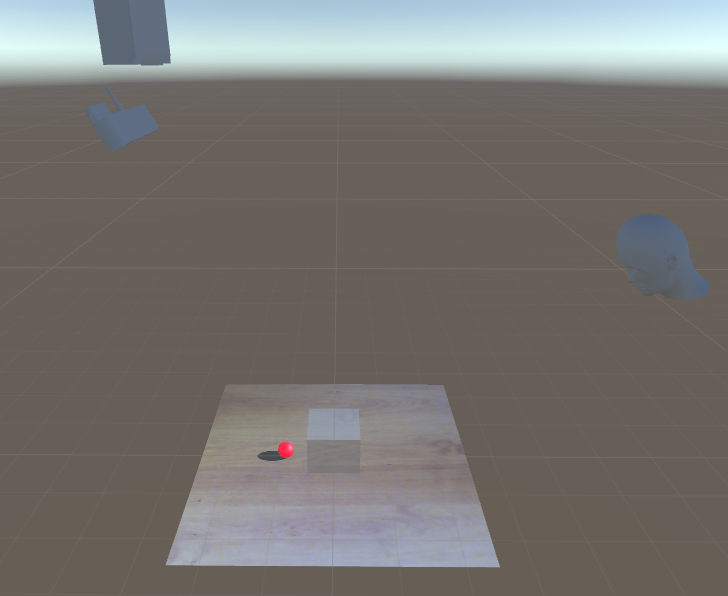
\includegraphics[width=0.65\linewidth]{images/unityscene}
\caption{Représentation du monde dans \texttt{Unity} - A droite la tête de l'utilisateur, au centre la table, en haut à gauche le couple caméra projecteur.}
\label{fig:unityrealworld}
\end{figure}

Le module \texttt{Unity} possède actuellement deux types de composants:
\begin{itemize}
\item Les composants modélisant les objets matériels du système de projection, correspondant aux différents dispositifs d'acquisition (caméras, projecteurs).
\item Les composants modélisant la partie logicielle, correspondant aux divers services de traitement fournis par \texttt{Nectar}.
\end{itemize}

Le fonctionnement d'un composant, peu importe ce qu'il modélise, reste le même. Dans un premier temps, ce dernier créer un client et essaie de se connecter à la base de données \texttt{Redis}, base dans laquelle tous les services de \texttt{Nectar} si tant est qu'ils produisent des données stockent ces dernières. Si \texttt{Redis} est déficient, la connexion échoue et il s'agit alors d'une erreur critique car cela signifie par la même occasion que \texttt{Nectar} n'a pas pu démarrer ses services. Dans un tel cas, le composant envoie une requête HTTP au serveur web communiquant avec le gestionnaire de processus \texttt{Eye} dans le but de redémarrer \texttt{Redis}. Si \texttt{Redis} est toujours déconnecté, un message d'erreur critique est remonté à l'utilisateur qui ne pourra utiliser aucun des composants du module jusqu'à ce que \texttt{Redis} soit de nouveau opérationnel. 

Une fois la connexion avec \texttt{Redis} établie, le composant, toujours par le biais d'une requête HTTP, questionne le serveur web sur l'état du service qu'il représente. Par exemple, le composant modélisant la caméra se renseignera sur l'état du service caméra. Si le service est hors ligne, une requête de démarrage peut être envoyée au serveur web qui la transmet instantanément à \texttt{Eye} afin de rendre opérationnel le service désiré. Si le service désiré n'existe pas ou ne peut être démarré, un message d'avertissement sur l'indisponibilité de ce dernier est remonté à l'utilisateur qui peut toutefois continuer à utiliser les autres composants du module ne dépendant pas de celui-ci. 
Lorsque le service est démarré, ou s'il était déjà en ligne, le composant peut finalement récupérer les données qu'il désire utiliser dans \texttt{Redis}. Pour ce faire, il est nécessaire que ce dernier en connaisse l'emplacement. \texttt{Redis} fonctionnant sur un système de clé-valeur comme expliqué section~\ref{sec:nectararchi}, une connaissance a priori de la clé est requise. C'est pourquoi chaque composant possède un ou plusieurs champs configurables par l'utilisateur pour indiquer les clés à utiliser afin de récupérer les données dans \texttt{Redis}. Par exemple, le composant caméra qui doit à la fois récupérer les paramètres intrinsèques, extrinsèques\footnote{\href{https://fr.wikipedia.org/wiki/Calibration_de_caméra}{Wikipédia - Calibration de caméra}} et le format des données produites par la caméra, possède trois champs configurables dans \texttt{Unity} permettant d'indiquer les clés de stockage dans \texttt{Redis}.\\

On peut observer, encadrés dans la Figure~\ref{fig:unity:plugin}, les trois points importants du module. 
\begin{itemize}
\item En vert est représentée la zone où les composants nécessaires à la création d'applications sont ajoutés afin d'en utiliser les fonctionnalités. Ici par exemple, nous utilisons une caméra, un projecteur et une caméra de profondeur rangés dans la catégorie \emph{Hardware}, un point de vue utilisateur \emph{UserPOV (Point Of View)} et différents services comme par exemple le suivi de feuille \emph{Paper Tracker}. Nous avons aussi ajouté à cette scène différents \emph{Renderer} permettant de visualiser les données acquises/générées par les dispositifs d'acquisition.
\item En rouge, on retrouve la zone où il va être possible de contrôler l'état des composants et, si besoin, de démarrer/redémarrer les services comme mentionné précédemment. Dans notre exemple, toujours Figure~\ref{fig:unity:plugin}, on peut observer le script de contrôle du composant projecteur. Ce script permet de spécifier quel type de dispositif on souhaite créer ; ici la valeur est \emph{PROJECTOR}. On peut également voir l'état interne du composant ; ici le composant est dans l'état \emph{WORKING}, ce qui signifie que ce dernier a réussi à se connecter à \texttt{Redis} et à récupérer les données dont il avait besoin pour fonctionner. On y retrouve aussi les clés où sont stockées lesdites données à récupérer, et un bouton permettant de démarrer/redémarrer le service en cas d'échec lors de l'initialisation.
\item En bleu, on peut voir la zone où les notifications de tout type (erreur, avertissement, fonctionnement) sont remontées à l'utilisateur lui indiquant constamment l'état des services et les problèmes détectés. Chaque notification commence par le nom du composant la générant suivi du message, afin de garder une certaine lisibilité.
\end{itemize}

\begin{figure}[H]
\centering
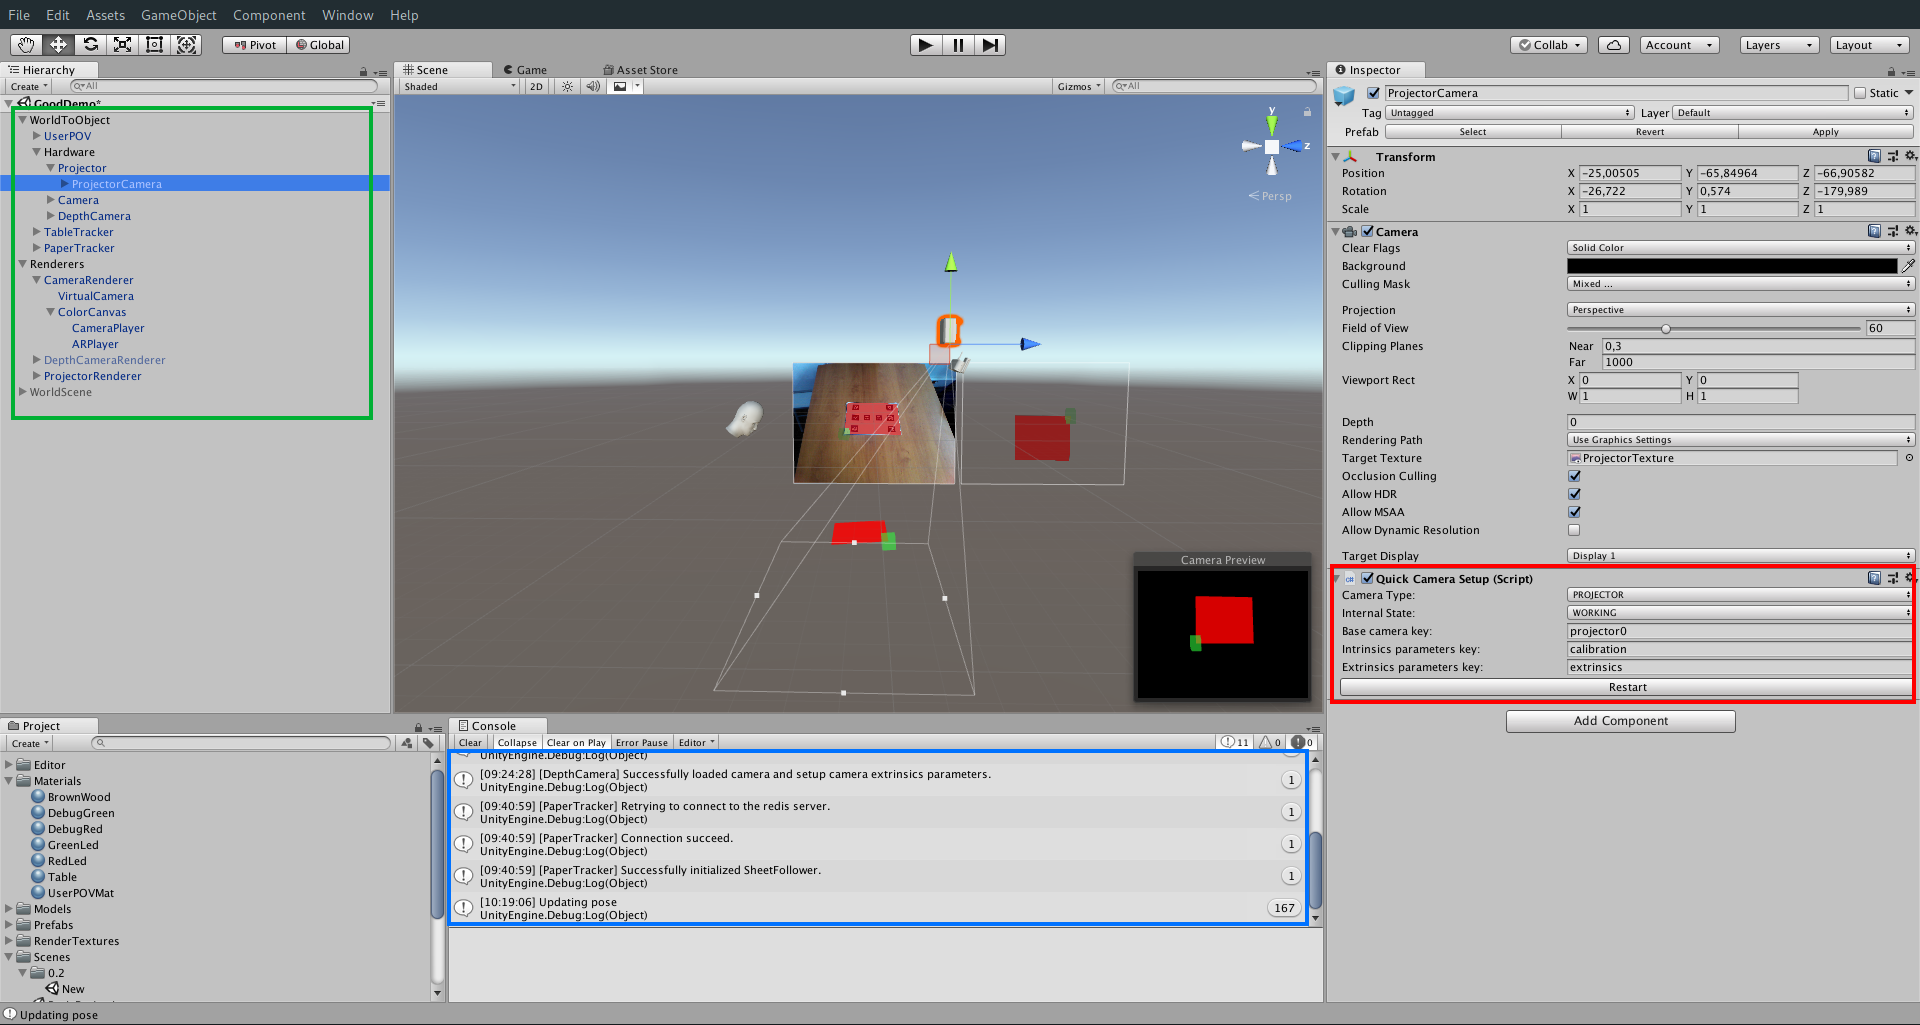
\includegraphics[width=\linewidth]{images/unity-plugin}
\caption{Vue globale du module \texttt{Unity} et de ses différents composants}
\label{fig:unity:plugin}
\end{figure}

Tous les composants et scripts ont été spécialement créés pour s'exécuter directement dans l'éditeur \texttt{Unity} afin de faciliter considérablement le développement pour les utilisateurs. Ainsi, il n'est pas nécessaire de construire et d'exécuter l'application pour avoir un retour sur la création en cours. Cela permet donc de gagner un temps précieux et d'accélérer le développement.

Le mode éditeur possède cependant quelques défauts majeurs qui ont requis une modification à la fois du module et à la fois des services \texttt{Nectar} afin de fonctionner correctement. 
En effet, à l'origine les services \texttt{Nectar} utilisaient le \emph{pipeline} événementiel de \texttt{Redis} pour qu'ils n'aient pas besoin d'effectuer de l'attente active et ainsi consommer 99\% des ressources, attendant indéfiniment de nouvelles données. Ce \emph{pipeline} permettait de souscrire à certaines clés, afin d'être notifié lorsque de nouvelles données étaient publiées sur ces dites clés. Ce \emph{pipeline} était très performant mais a posé quelques problèmes avec le fonctionnement en éditeur de \texttt{Unity}. En effet, en mode éditeur, les performances sont très amoindries\footnote{\href{https://forum.unity.com/threads/low-performance-in-editor-but-working-fine-in-build.489030/}{Unity : Low performance in editor}} et ce dernier n'était donc pas capable de traiter suffisamment vite les évènements reçus. Les données s'accumulaient sans être consommées par les clients. \texttt{Redis} stockant ces données directement dans la mémoire vive comme expliqué section~\ref{sec:nectararchi}, l'accumulation causait une surcharge et mettait en péril toute la base. Il était donc nécessaire de couper la connexion avec le client du composant se trouvant dans l'incapacité de consommer ces données.

Pour que cette version puisse fonctionner correctement, nous avons décidé d'ajouter à tous les services \texttt{Nectar} la possibilité, ou non, d'utiliser le pipeline événementiel. Cette option permet ainsi d'utiliser le pipeline classique où les données ne s'accumulent pas mais écrasent les anciennes déjà existantes. Du côté du module, le même comportement a été implémenté pour tous les composants fonctionnant directement dans l'éditeur afin de pouvoir utiliser les services. Cette solution résout bel et bien le problème de fonctionnement en mode éditeur mais comporte encore quelques défauts.

Le pipeline ne se basant plus sur des événements, la seule façon de mettre à jour les composants est d'utiliser la boucle principale gérée par \texttt{Unity}. De ce fait, comme on peut le voir dans l'ordre d'exécution des différentes fonctions de \texttt{Unity} que vous trouverez en Annexe~\hyperref[annexe:unity]{3}, celles de la boucle que nous pouvons utiliser sont celles de mise à jour (\emph{Update}). Le problème avec ces fonctions réside dans le fait que, lors de l'utilisation dans l'éditeur, celles-ci ne sont pas systématiquement appelées (comme elles le seraient en mode jeu ou quand l'application est construire puis exécutée) afin d'alléger la consommation des ressources et permettre d'avoir un meilleur confort de développement. Ainsi, il en résulte que les composants ne se mettent à jour que lorsque \texttt{Unity} reçoit des événements et décide de se mettre à jour, comme c'est le cas si une valeur telle que la position d'un objet est modifiée dans l'éditeur. Actuellement ce défaut de comportement est toujours présent dans le module mais des pistes d'améliorations sont envisagées section~\ref{sec:unity:bilan}.\\

Une des dernières difficultés rencontrées durant le développement du module \texttt{Unity} a été la gestion des formats de données envoyées par les différents services et plus spécifiquement les matrices. Chaque service étant indépendant, les données qu'il envoie ne sont pas toujours au même format que celui attendu par \texttt{Unity}. En effet, si on prend le cas des matrices, celles du moteur 3D de \texttt{Unity} sont dites \emph{row major} ce qui signifie que les données sont indexées en fonction des lignes alors que celles du moteur 3D de \texttt{Processing} sont dites \emph{column major}, et donc indexées en fonction des colonnes. Il a donc fallu appliquer des traitements spécifiques en fonction des données reçues afin d'obtenir une visualisation cohérente de ces dernières.

Une fois la majeure partie des problèmes du module résolue, il était temps d'enfiler le costume d'utilisateur développeur client de \texttt{RealityTech} et d'expérimenter le développement d'une application de réalité augmentée spatiale avec ce module. Vous trouverez les détails de ce développement section~\ref{sec:unity:appli}.

\section{Illusion de projection}
\label{sec:unity:appli}

Après voir achevé la première version du module \texttt{Unity}, dans une optique de test de ce dernier mais aussi dans le but de proposer une preuve de concept, j'ai été chargé de développer une application simulant une illusion de projection afin de créer un effet de fausse transparence. Cette preuve de concept avait été demandée par de potentiels clients de la société, rencontrés au \texttt{Laval Virtual}, afin qu'ils puissent effectuer de la présentation de produit interactive et plus spécifiquement de la présentation de parfum. Ceci est typiquement un cas d'utilisation auquel il était difficile de répondre avec la version \texttt{Processing} du kit de développement car elle ne permettait pas facilement de manipuler des objets 3D, de gérer la transparence, de faire le rendu de la scène en plusieurs étapes etc. 

Afin de pouvoir créer une illusion de projection, il est nécessaire d'avoir une connaissance a priori de la surface de projection, permettant d'appliquer les déformations nécessaires à la géométrie à projeter. Grâce à la représentation du monde réel directement dans \texttt{Unity}, nous pouvons aisément disposer des éléments de géométrie qui nous sont nécessaires (Figure~\ref{fig:realvsunity}). Ainsi, seuls les éléments purement virtuels à projeter sont à rajouter dans la scène 3D.

\begin{figure}[H]
\centering
	\subfloat[Photographie de la scène]{
      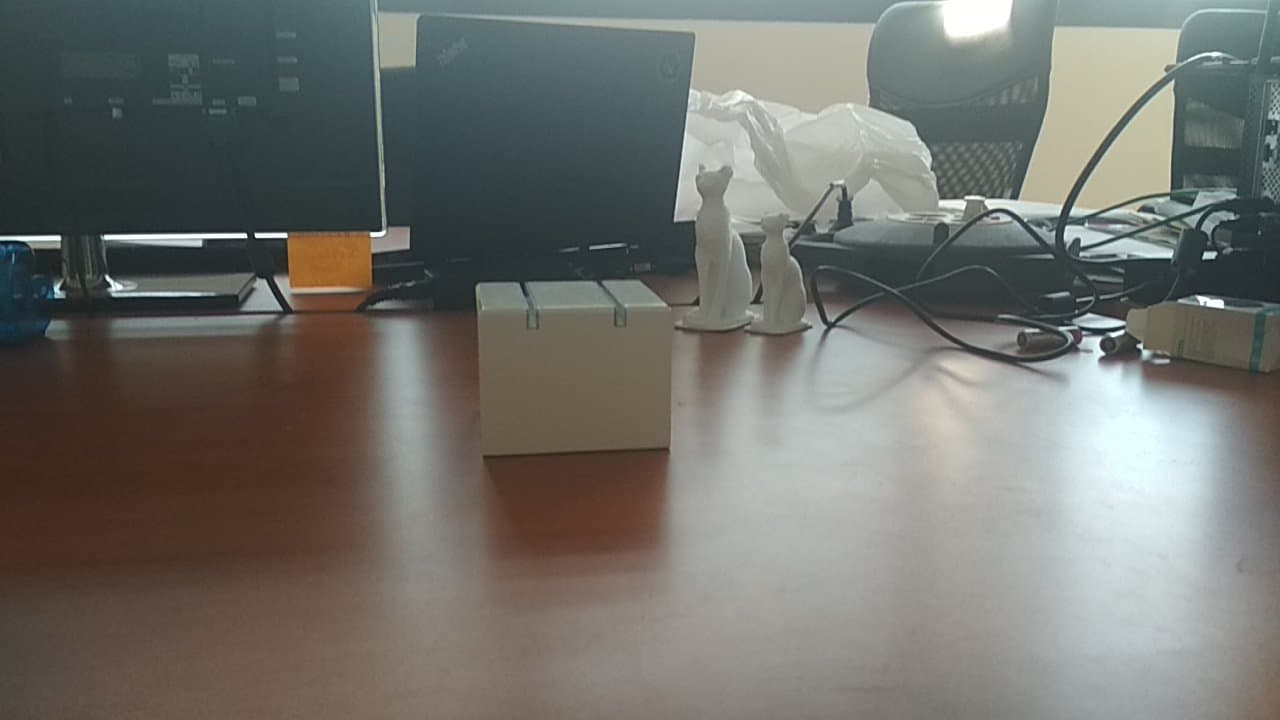
\includegraphics[width=0.45\textwidth, trim = 7.5 2.5cm 7.5cm 5cm, clip]{images/Unity-Projection-RealReal}
      \label{sub:unity:app:realworldview}
      }
     \subfloat[Représentation dans \texttt{Unity}]{
      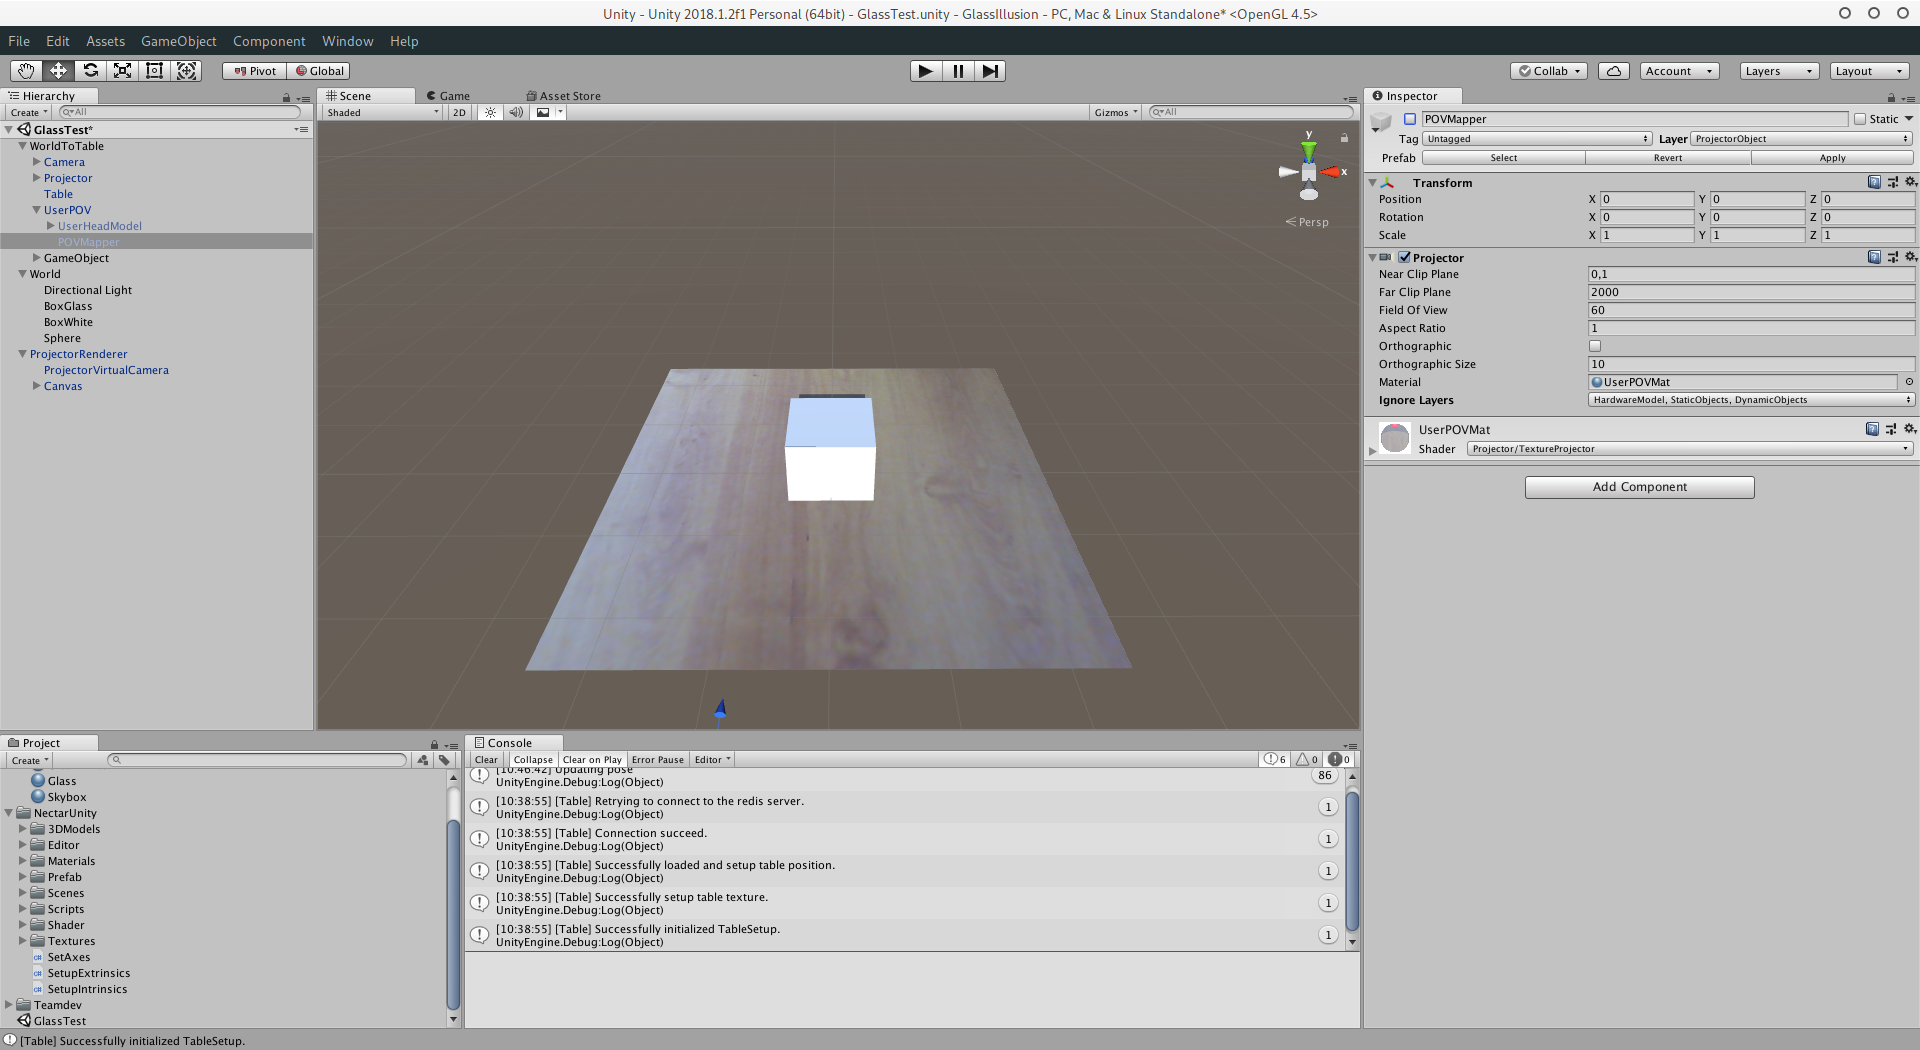
\includegraphics[width=0.45\textwidth, trim = 12cm 12cm 20cm 4.5cm, clip]{images/Unity-Projection-UserPOV-NoMap}
      \label{sub:unity:app:unityview}
      }
\caption{Monde réel et sa représentation dans \texttt{Unity}}
\label{fig:realvsunity}
\end{figure}

Aussi, une illusion de projection ne fonctionne que pour un point de vue donnée (Figure~\ref{fig:projpov}) car la perception de la géométrie du monde réel diffère selon ce dernier. Les déformations à appliquer ne seront donc pas les mêmes selon le point de vue.

\begin{figure}[H]
\centering
	\subfloat[Bon point de vue] {
	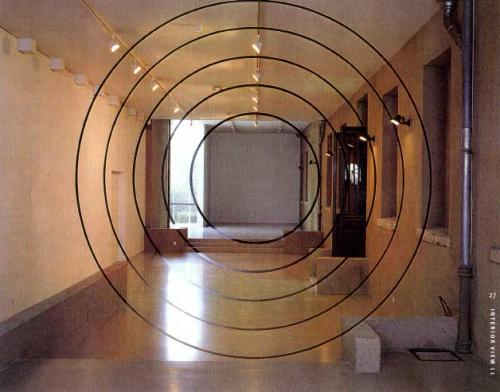
\includegraphics[width=0.45\textwidth]{images/proj-illu-good-pov}
	\label{sub:ilu:badpov}
	}
	\subfloat[Mauvais point de vue] {
	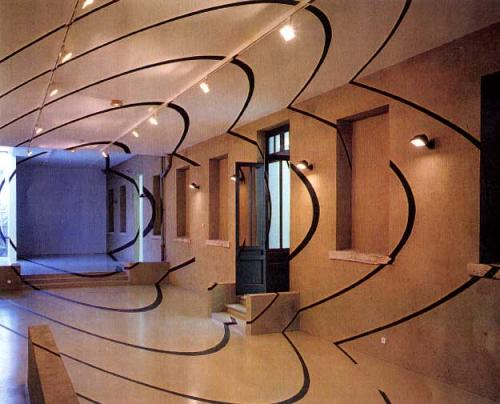
\includegraphics[width=0.42\textwidth]{images/proj-illu-bad-pov}
	\label{sub:ilu:goodpov}
	}
\caption{Illusion de projection}
\label{fig:projpov}
\end{figure}

Ainsi, les éléments requis pour commencer à créer notre illusion sont: la modélisation du monde réel, ici la table et sa texture (pour que l'effet de transparence ait du sens) ainsi que le flacon de parfum que l'on souhaite faire apparaître transparent, la position de l'utilisateur observant la scène et le point de vue du projecteur. Tous ces éléments font partie du module de développement, il a donc suffit de les ajouter à la scène pour en obtenir la représentation (Figure~\ref{fig:unity:projscene}).
De plus, afin de vérifier la validité de l'effet nous avons choisi d'ajouter une sphère virtuelle rouge derrière le flacon, invisible du point de vue de l'utilisateur, de sorte à ce qu'elle apparaisse lorsque l'effet de transparence sera mis en place.

\textbf{Note:} Dans notre cas, nous n'avions pas le modèle 3D du parfum imprimé à disposition, nous avons donc choisi de le remplacer par un cube cependant cela n'a aucun impact sur la simulation de l'effet de transparence.

\begin{figure}[H]
\centering
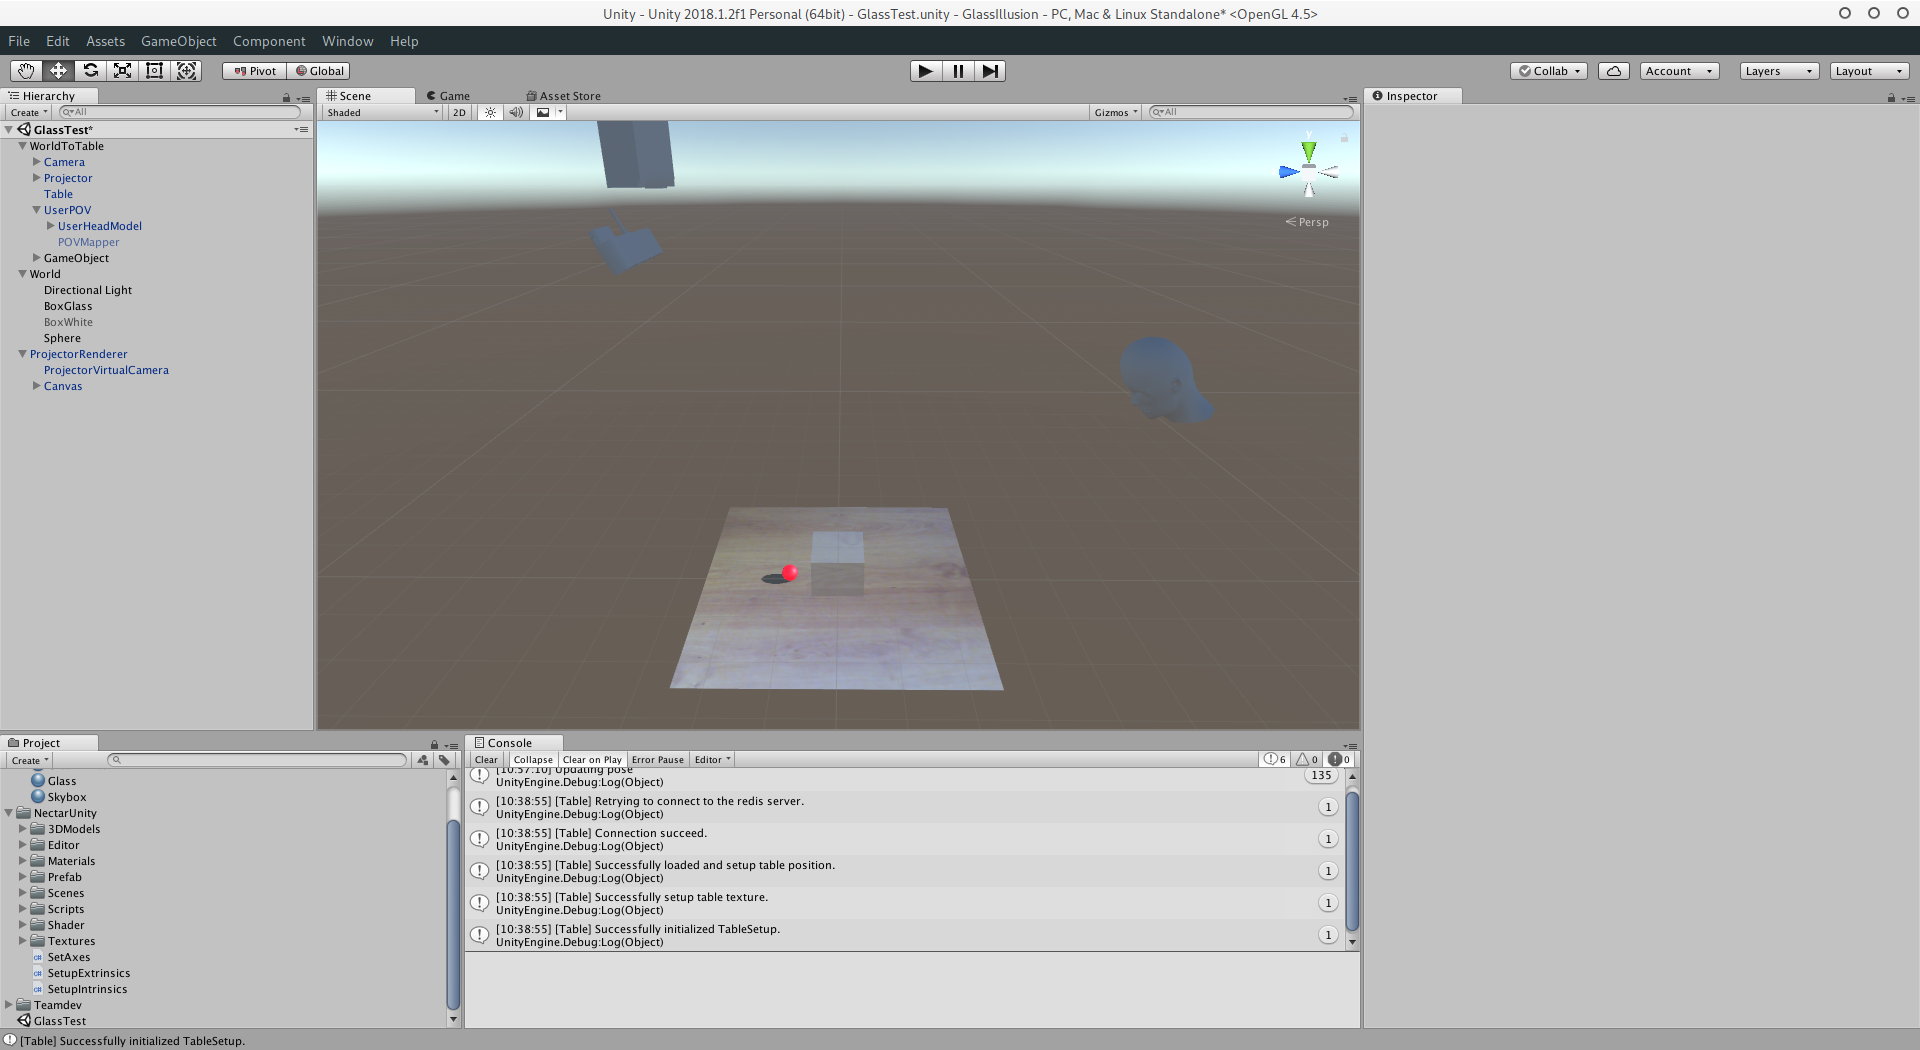
\includegraphics[width=0.75\linewidth, trim = 12cm 12cm 20cm 4.5cm, clip]{images/Unity-Projection-RealScene}
\caption{Scène modélisée pour tester l'effet de transparence}
\label{fig:unity:projscene}
\end{figure}

Pour réaliser un tel effet, le rendu se fait en plusieurs étapes. Dans un premier temps, le rendu de la scène est effectué depuis le point de vue de l'utilisateur avec l'objet d'intérêt transparent et en ignorant sa représentation physique (Figure~\ref{sub:unity:proj:userpov:transparency}). Ce rendu se fait \emph{offscreen} et est ensuite récupéré dans une texture. La prochaine étape consiste à utiliser la texture ainsi créée et à la projeter sur la géométrie de la scène, comprenant cette fois ci l'objet physique, afin qu'elle subisse les déformations adéquates pour créer l'illusion (Figure~\ref{sub:unity:proj:userpov:nomap},~\ref{sub:unity:proj:nopov:map} et~\ref{sub:unity:proj:userpov:map}). On peut observer qu'une ombre est apparue. En effet, pour renforcer l'effet qu'allait produire l'illusion nous avons choisi d'ajouter une lumière pour obtenir des ombres cependant nous avons oublié d'activer leurs rendus pour les objets transparents. Pour pouvoir projeter cette texture sur la scène, il a fallu implémenter un principe de vidéo projecteur. Ce vidéo projecteur ne devait projeter la texture que sur le modèle physique et non pas sur sa représentation transparente. Enfin, la dernière étape consiste à faire le rendu de la scène, avec la texture projetée sur la géométrie vue par le projecteur (Figure~\ref{sub:unity:proj:projectorpov:map}) pour ainsi pouvoir projeter ce résultat dans le monde réel. 

Pour des raisons logistiques, je n'ai malheureusement pas eu l'occasion de prendre une photo de ce dispositif en train de fonctionner.

\begin{figure}[H]
\centering
	\subfloat[Point de vue utilisateur - Objet transparent] {
		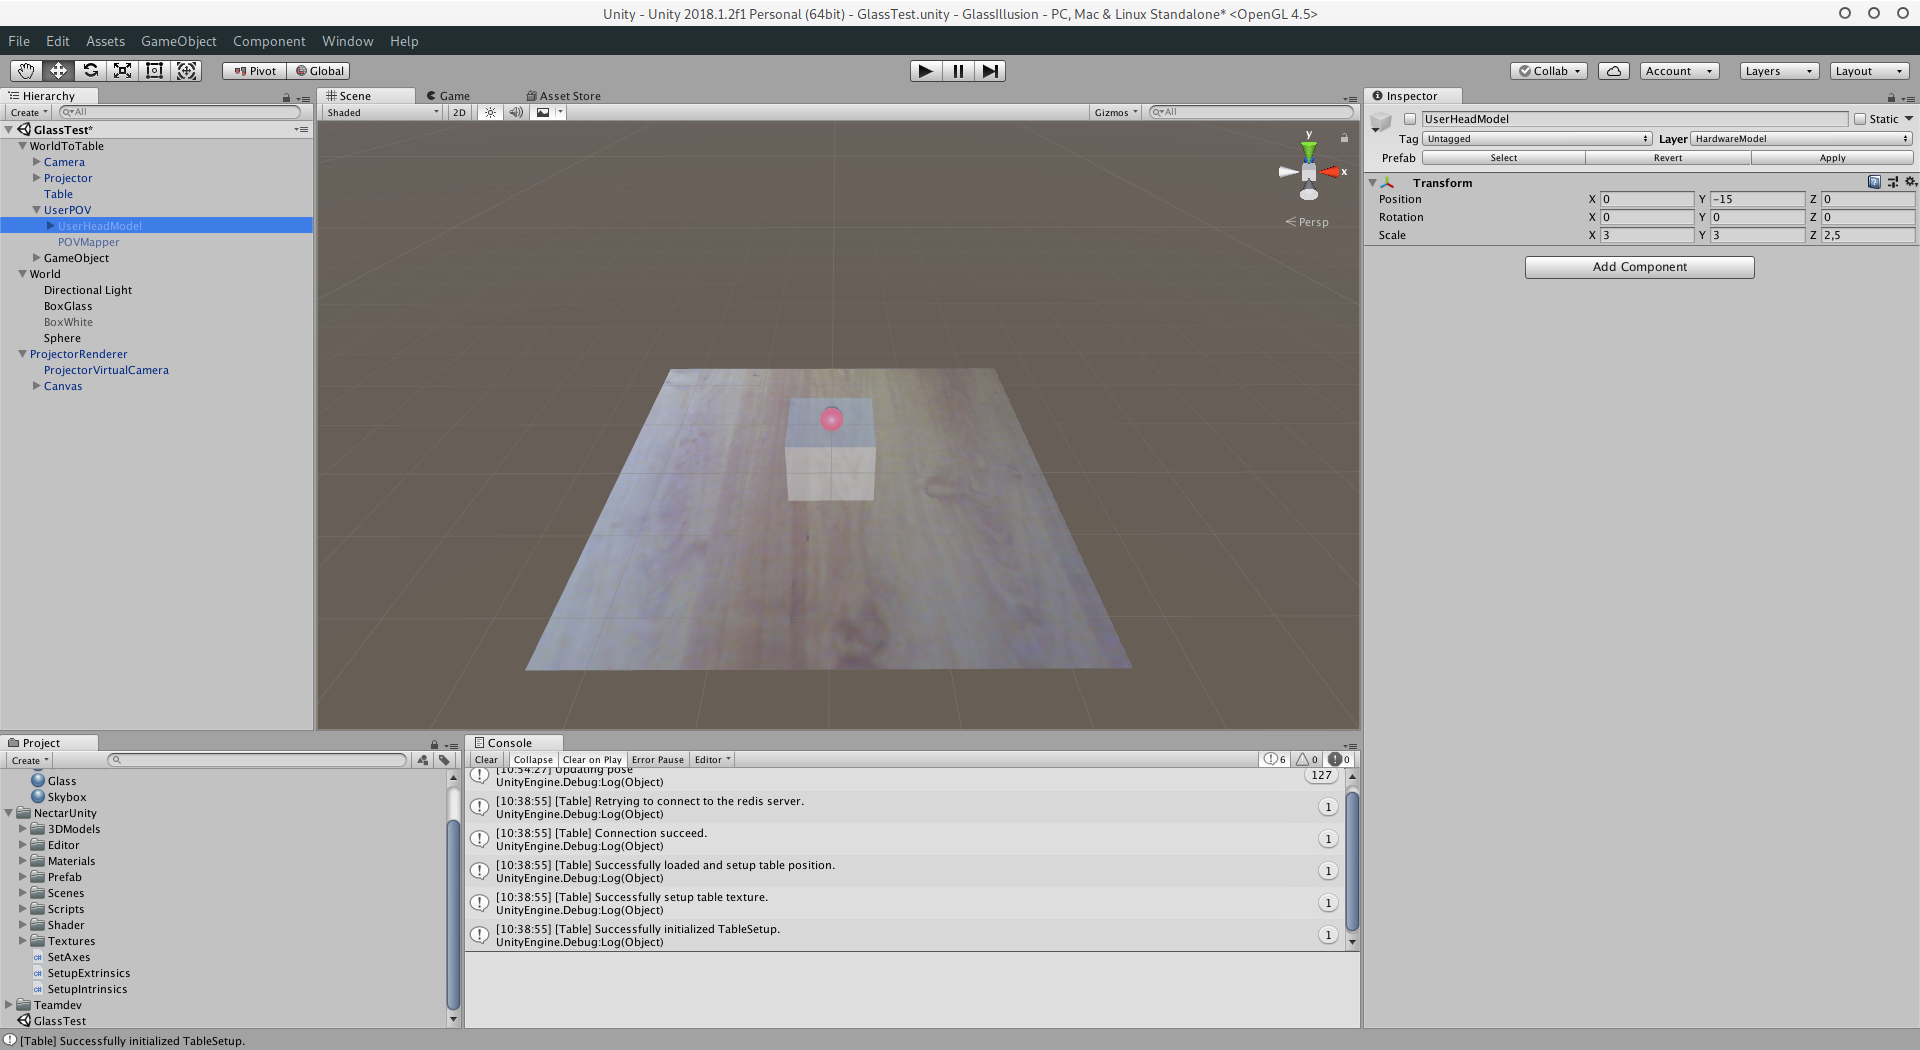
\includegraphics[width=0.4\textwidth, trim = 12cm 12cm 20cm 4.5cm, clip]{images/Unity-Projection-UserPOV-RealScene}
		\label{sub:unity:proj:userpov:transparency}
	}
	\subfloat[Point de vue utilisateur - Objet physique] {
		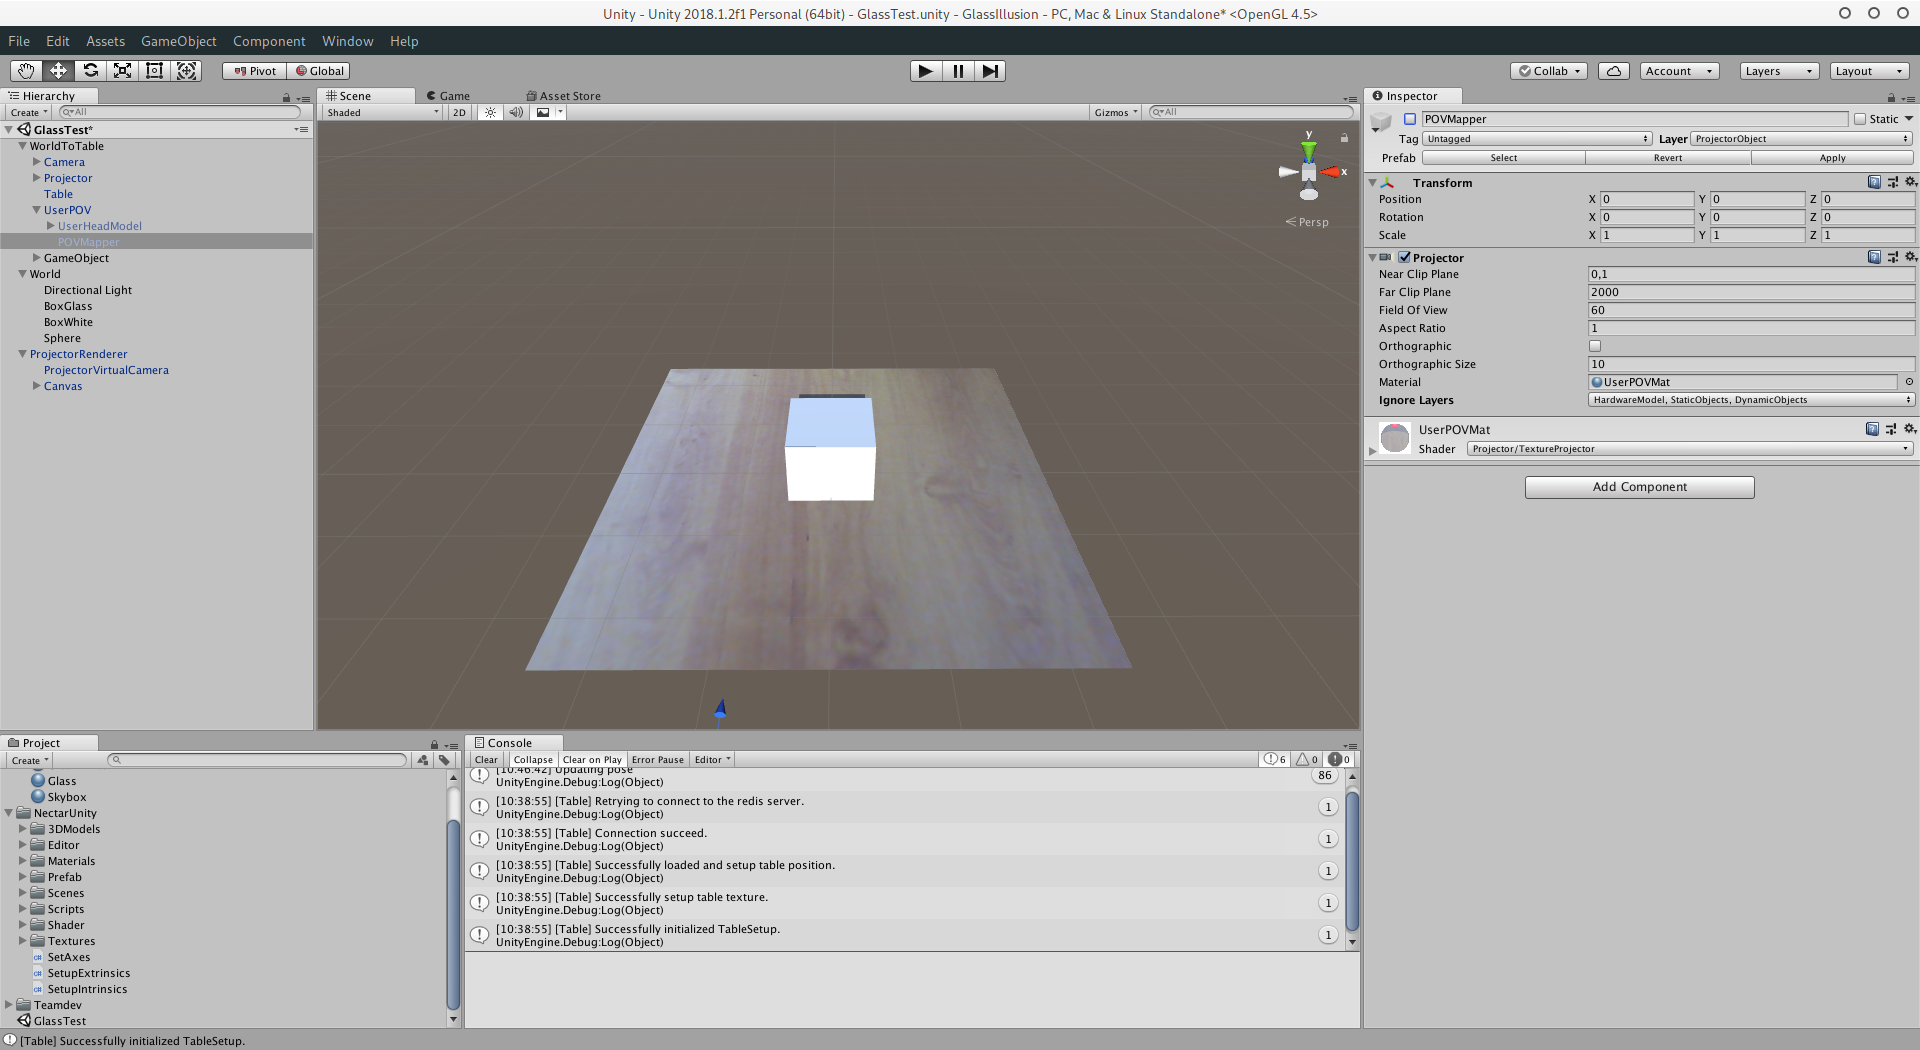
\includegraphics[width=0.4\textwidth, trim = 12cm 12cm 20cm 4.5cm, clip]{images/Unity-Projection-UserPOV-NoMap}
		\label{sub:unity:proj:userpov:nomap}
	}\\
	\subfloat[Point de vue différent - Objet physique + texture projetée] {
		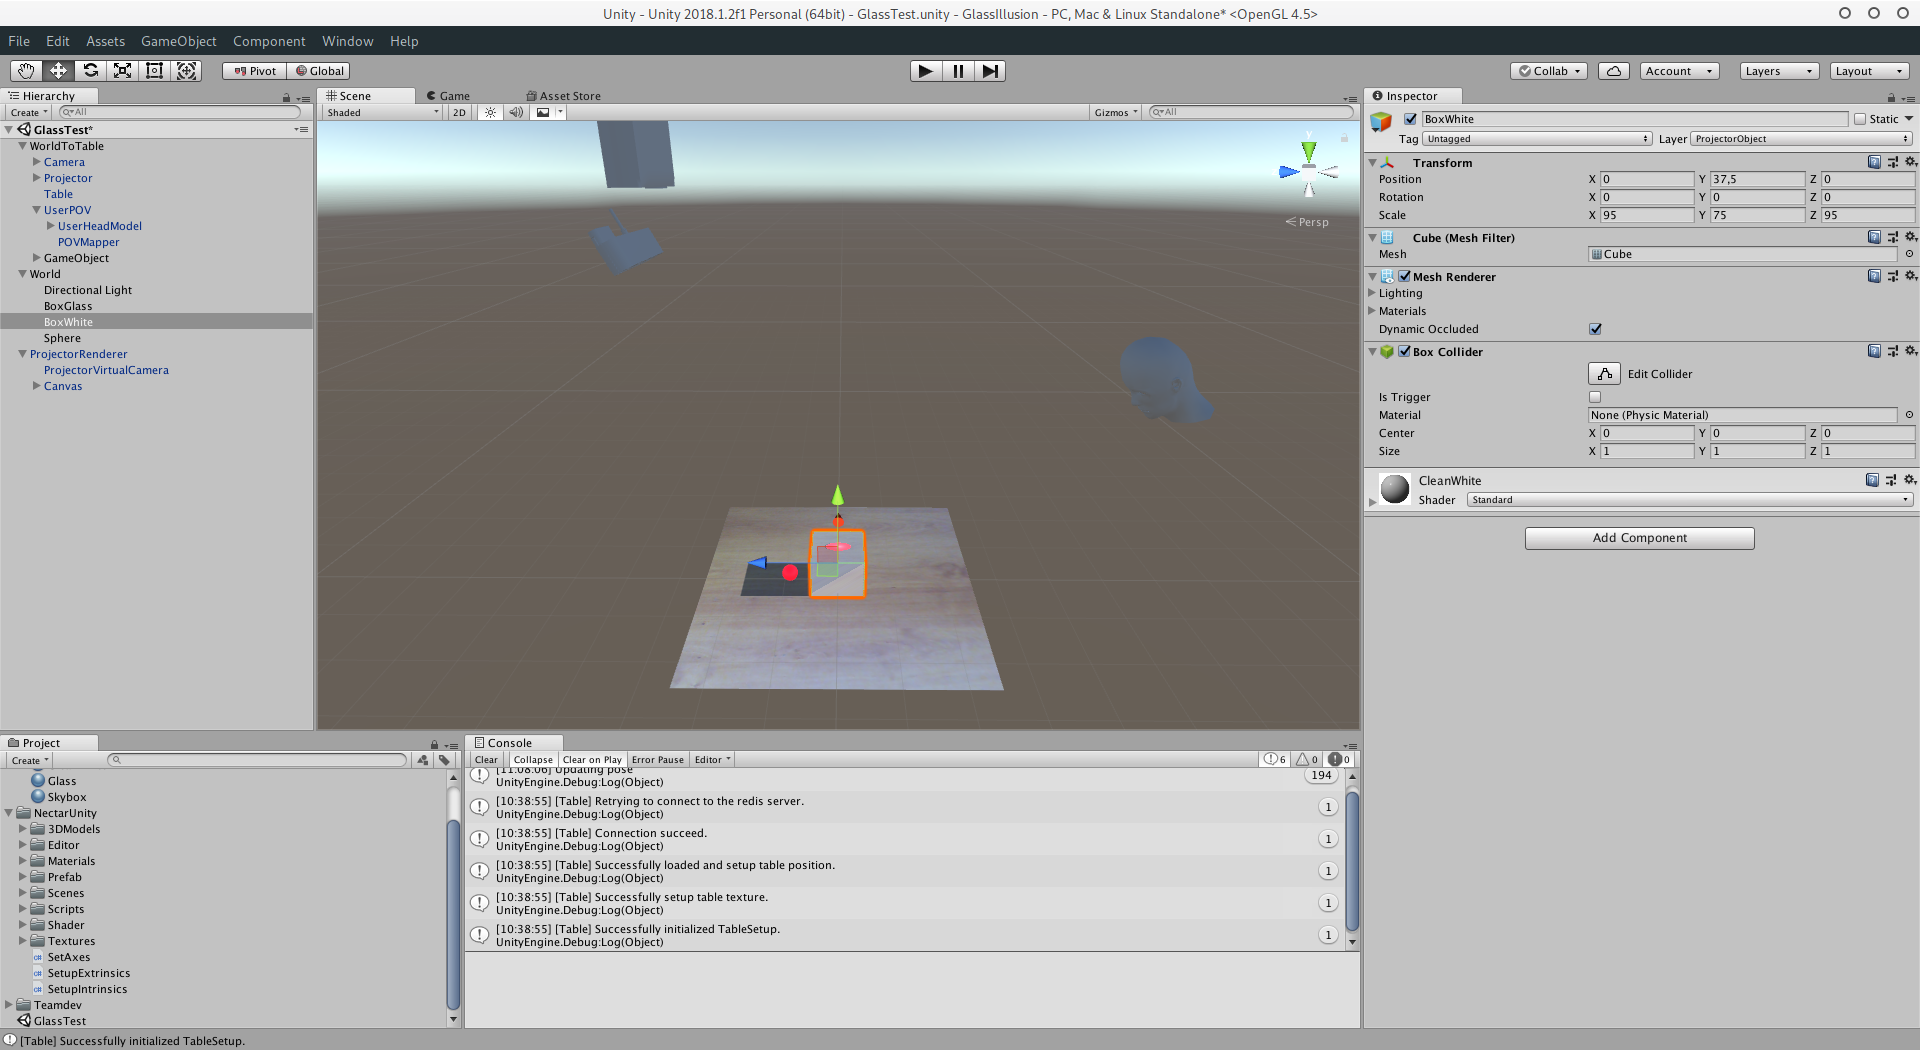
\includegraphics[width=0.4\textwidth, trim = 12cm 12cm 20cm 4.5cm, clip]{images/Unity-Projection-RealSceneWithMap}
		\label{sub:unity:proj:nopov:map}
	}
	\subfloat[Point de vue utilisateur - Objet physique + texture projetée] {
		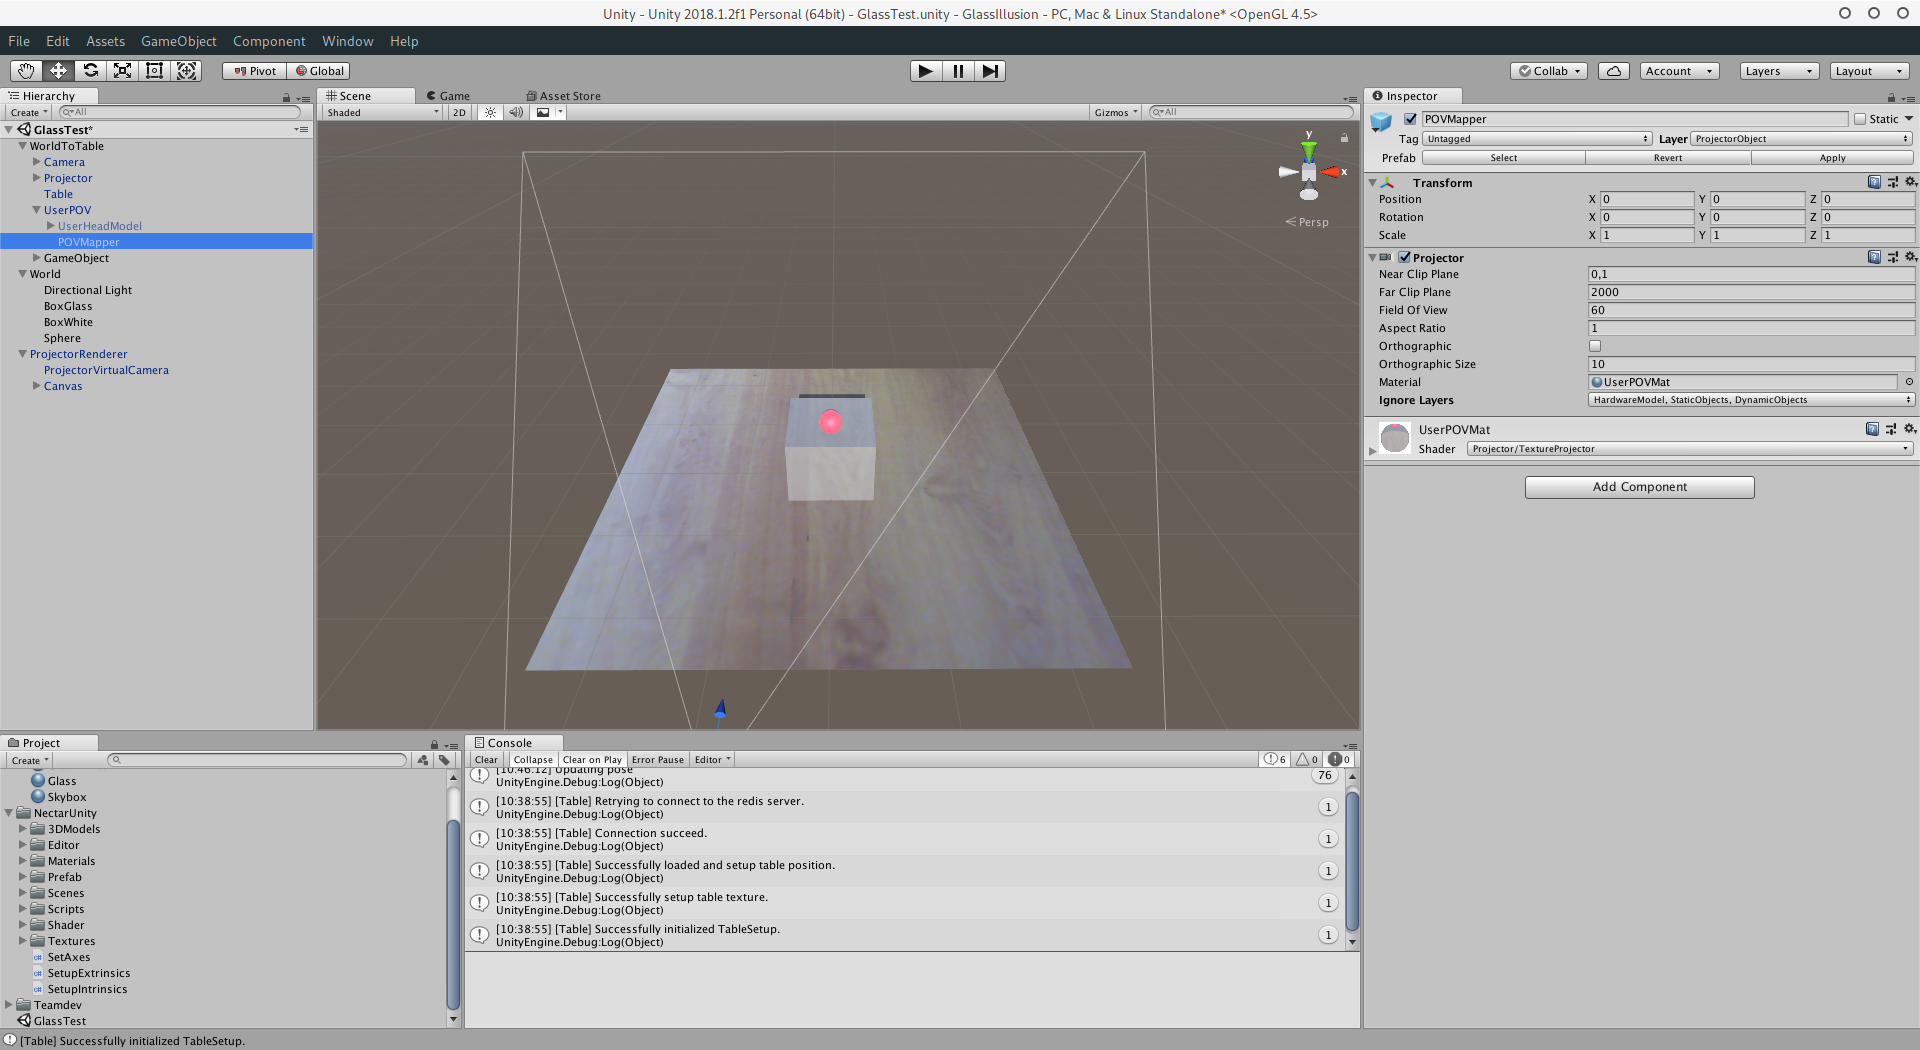
\includegraphics[width=0.4\textwidth, trim = 12cm 12cm 20cm 4.5cm, clip]{images/Unity-Projection-UserPOV-Mapper}
		\label{sub:unity:proj:userpov:map}
	}\\
	\subfloat[Point de vue projecteur - Objet physique + texture projetée] {
		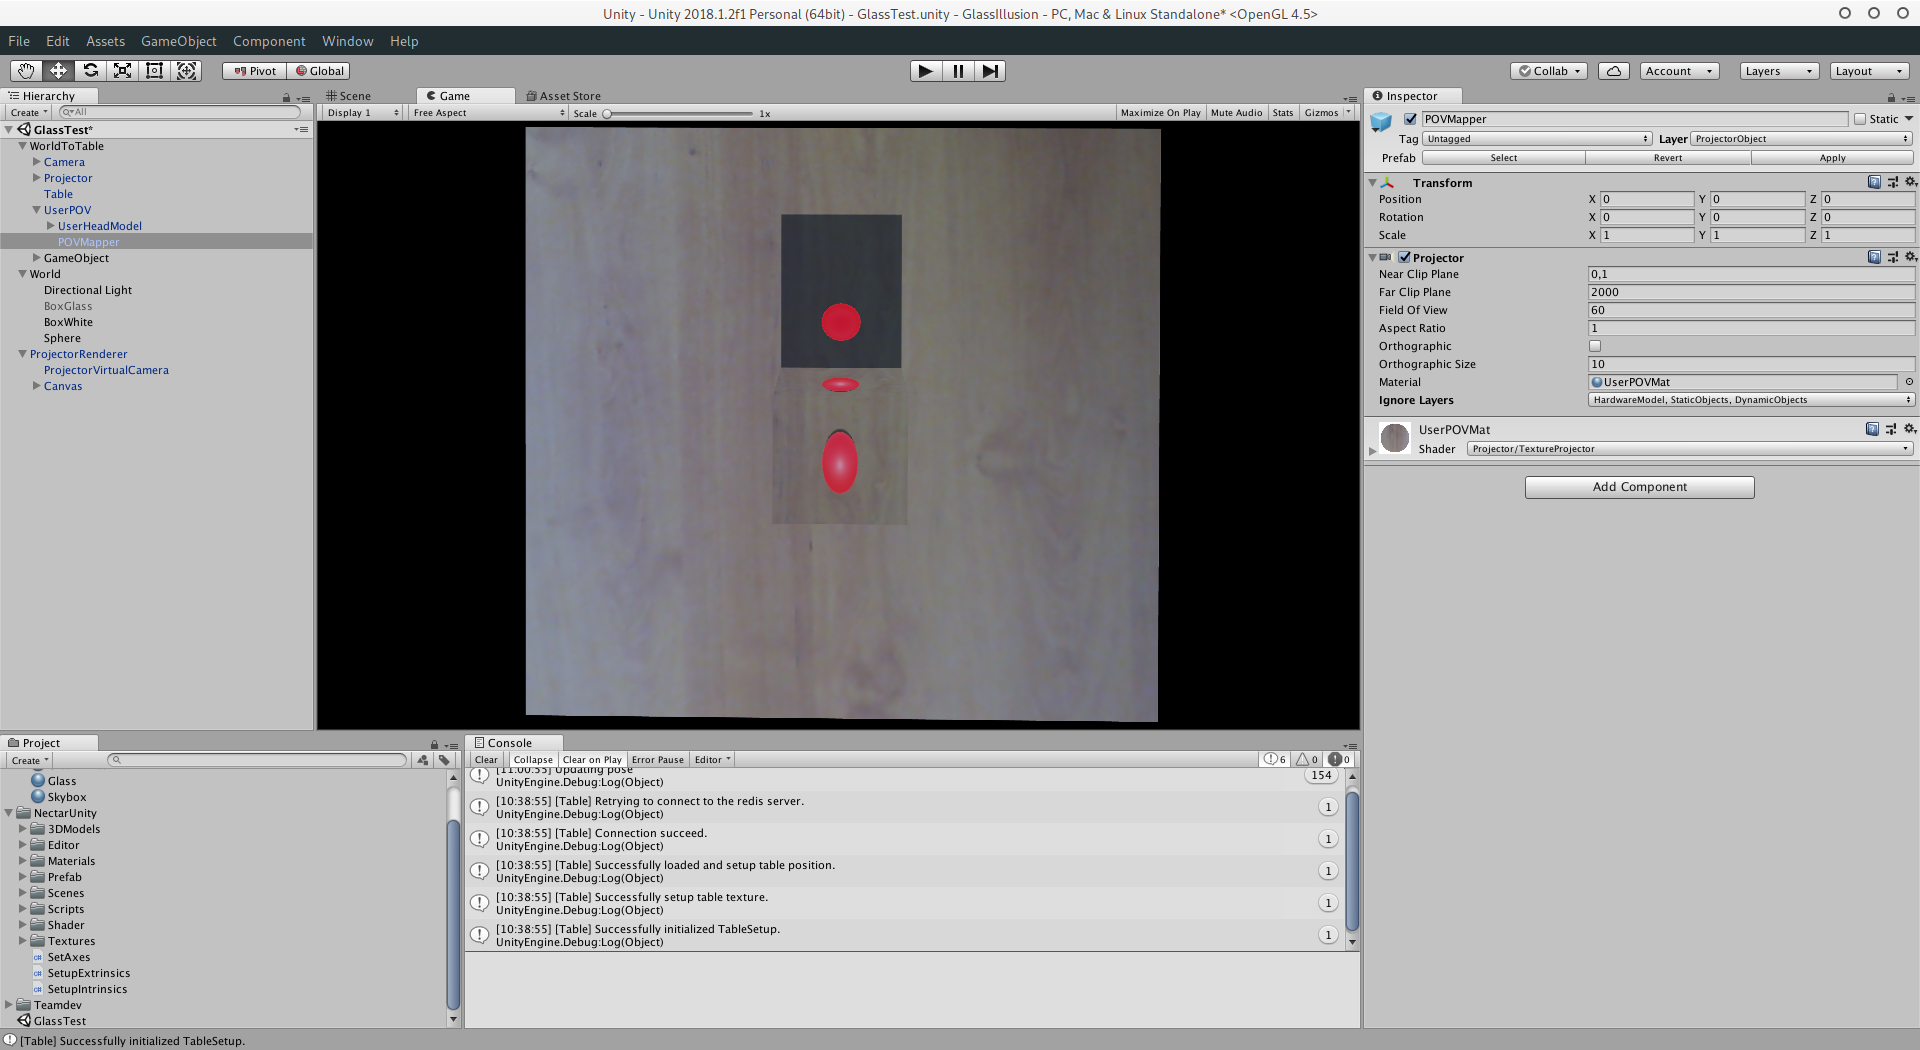
\includegraphics[width=0.4\textwidth, trim = 12cm 12cm 20cm 4.5cm, clip]{images/Unity-Projection-ProjectorPOV}
		\label{sub:unity:proj:projectorpov:map}
	}
\caption{Étapes de la création de l'illusion de projection}
\label{fig:unity:illuproj}
\end{figure}

Dans l'état actuel des choses, l'illusion est encore incomplète pour plusieurs raisons. La première étant que nous utilisons actuellement un système composé d'un seul projecteur positionné au dessus de l'objet. Il est de ce fait impossible de couvrir toute la surface du cube ou de n'importe quel objet en général avec de la projection. Plus précisément, dans notre cas, nous ne pouvons projeter que sur la face supérieure et arrière du cube. Aussi pour renforcer l'illusion, il aurait été intéressant d'utiliser la caméra ainsi que la caméra de profondeur du système pour créer des représentations 3D virtuelles des éléments du monde réel. Ces objets 3D auraient ainsi pu être intégrés à la scène dans \texttt{Unity} et donc à l'illusion de transparence. Par exemple, si une personne décidait de passer sa main derrière le cube physique non transparent dans le monde réel, il aurait été possible d'afficher cette dernière en transparence derrière le cube, donnant ainsi l'illusion que le cube est réellement transparent.

\section{Bilan}
\label{sec:unity:bilan}
La version \texttt{Unity} du kit pour le développement d'applications de réalité augmentée spatiale offre un confort sans précédent. Le coût en développement (du module, de l'architecture en microservices etc.) est largement contrebalancé par les multiples possibilités offertes par ce moteur. De plus, le module répond de façon assez complète aux objectifs que nous nous étions fixés que ce soit en termes de performance ou d'expérience pour l'utilisateur développeur.

Le fonctionnement en mode éditeur apporte un vrai plus dont nous avons pu ressentir l'effet lors du développement de l'application dont il est question section~\ref{sec:unity:appli}. Toutefois, la nécessité de générer des événements pour qu'\texttt{Unity} mettent à jour les composants reste pénible. Pour pallier à ce problème, nous avons imaginé une nouvelle version des microservices utilisant de nouveau le pipeline évènementiel de \texttt{Redis}, où ces derniers ne publient plus les données qu'ils génèrent mais plutôt une notification au format \texttt{JSON}\cite{crockford2006application} très légère, ne risquant donc pas de surcharger la RAM et permettant d'indiquer aux services que des nouvelles données sont disponibles. On peut ainsi résoudre le problème de la surcharge mémoire et de l'attente active. Cette version fera l'objet des tâches à effectuer durant le dernier mois de stage.

Par ailleurs, la gestion des clés pour accéder aux données dans le module est très peu pratique et en complexifie l'utilisation sans qu'il n'y ai aucun bénéfice pour l'utilisateur. Une solution à ce problème aurait été de supprimer la gestion des clés dans \texttt{Unity} et de l'exporter sur le serveur web. Ainsi, lors d'une requête de démarrage d'un service, le serveur web en plus de démarrer ce service, pourrait envoyer à \texttt{Unity}, une réponse contenant la clé où ce dernier publie ses données. La gestion des clés deviendrait alors totalement invisible pour l'utilisateur du module ce qui lui permettrait de concentrer ses efforts sur le contenu de l'application.

Pour finir, la représentation du monde physique, offre un réel avantage au développeur ce qui lui permet de concentrer ses efforts sur la création de contenu en adéquation avec celui ci.